\newpage
\section{Countermeasure}
\begin{figure}[!ht]
\begin{center}
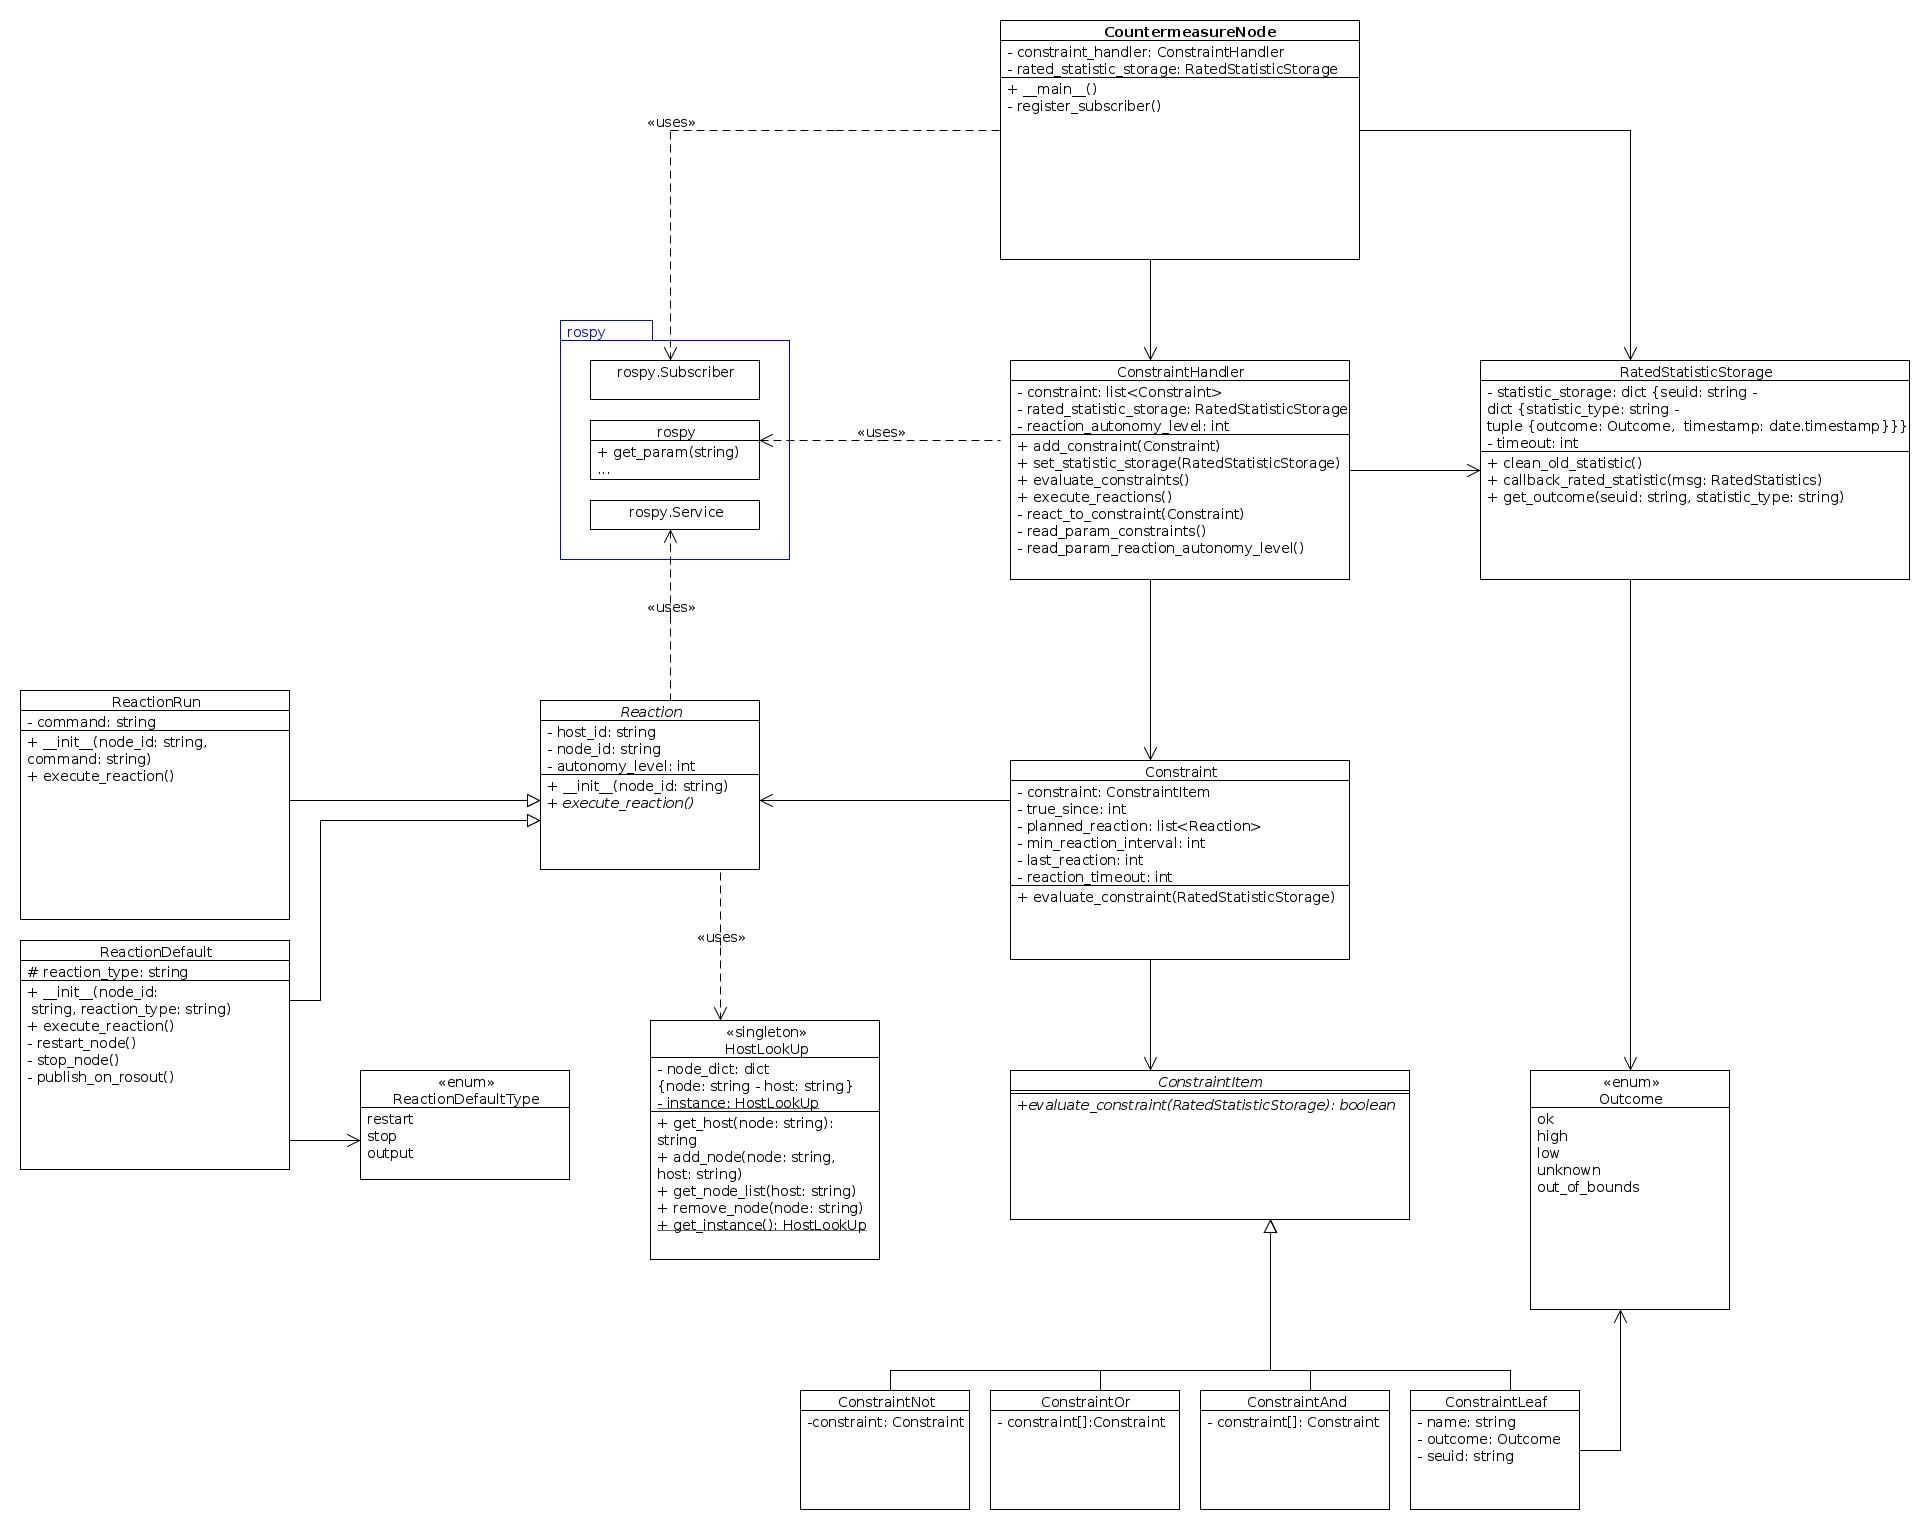
\includegraphics[width=1.0\linewidth]{./diagram_pictures/reactor.jpg}
\caption{The UML diagram of the countermeasure package}
\end{center}
\end{figure}

\mbox{}

\newpage


\subsection{CountermeasureNode}
a ROS node. Evaluates incoming rated statistics with a list of constraints. If those constraints turn out to be true appropriate action is taken.
\subsubsection{Attributes}
\begin{itemize}
	\item \textbf{ private ConstraintHandler constraint\_handler}\\
		the handler for all constraints
	\item \textbf{ private RatedStatisticStorage rated\_statistic\_storage}\\
		the storage of all incoming rated statistic
\end{itemize}
\subsubsection{Methods}
\begin{itemize}
	\item \textbf{ public void \_\_main\_\_() }\\\\
		periodically (threads) evaluates the constraints and cleans old statistics
	\item \textbf{ private void register\_subscriber() }\\
		registers to the rated statistics
\end{itemize}



\subsection{ConstraintHandler}
Manages all constraints, checks if they are true and executes appropriate reactions if neccessary.

\subsubsection{Attributes}
\begin{itemize}
	\item \textbf{ private list<Constraint> constraint }\\
		contains a list of all constraints
	\item \textbf{ private  RatedStatisticStorage rated\_statistic\_storage }\\
		contains all incoming rated statistic
	\item \textbf{ private  int reaction\_autonomy\_level }\\
		only reactions with an autonomy\_level <= reaction\_autonomy\_level get executed
\end{itemize}
\subsubsection{Methods}
\begin{itemize}
	\item \textbf{ public void add\_constraint(Constraint)  }\\
		adds an constraint to this list
	\item \textbf{ public void set\_statistic(RatedStatisticStorage)  }\\
		sets the Statistic to use. Should only be needed on initialisation
	\item \textbf{ public void evaluate\_constraints()  }\\
		evaluates every constraint
	\item \textbf{ public void execute\_reactions()  }\\
		checks if there are any new reactions to do and executes them.
	\item \textbf{ private void react\_to\_constraint(Constraint)  }\\
		executes an single Reaction and updates the attributes of the Constraint
	\item \textbf{ private void read\_param\_constraints()  }\\
		reads all constraints from the parameter server
	\item \textbf{ private void read\_param\_reaction\_autonomy\_level()  }\\
		reads the reaction\_autonomy\_level from the parameter server
\end{itemize}


\subsection{RatedStatisticStorage}
A database which contains the current state of all rated statistics.
\subsubsection{Attributes}
\begin{itemize}
	\item \textbf{ private dict\{string seuid - dict\{string statistic\_type - tuple\{Outcome outcome,date.timestamp timestamp\}\}\} statistic\_dict }\\
		a dictionary containing all rated statistic information with their outcome and an timestamp when they got added / updated to the dictionary.
	\item \textbf{ private int timeout }\\
		the timeout after which an item in ratedstatistic is declared too old and should be removed from the dict.
\end{itemize}
\subsubsection{Methods}
\begin{itemize}
	\item \textbf{ public void clean\_old\_statistic() }\\
		checks the complete dictionary for statistics older than timeout seconds and removes them.
	\item \textbf{ public void callback\_rated\_statistic(RatedStatistics msg) }\\
		callback for incoming rated statistics. adds them to the dictionary or removes items from the dictionary if the rated statistic says that its within bounds again. 
	\item \textbf{ public Outcome get\_outcome(string seuid, string statistic\_type) }\\
		returns the outcome of the specific seuid and statistic\_type.
\end{itemize}

\subsection{Constraint }
contains the whole constraint with corresponding reactions.


\subsubsection{Attributes}
\begin{itemize}
	\item \textbf{ private ConstraintItem constraint }\\
	first constraint in the chain of ConstraintItems.
	\item \textbf{ private int true\_since }\\
	epoch time in milliseconds since the constraint is true,
	if the constraint is not true it is 0
	\item \textbf{ private list<Reaction> planned\_reaction }\\
	an list of reactions that should be executed if the constraint has been true longer than min\_reaction\_interval milliseconds
	\item \textbf{ private int min\_reaction\_interval }\\
	the minimum time needed in ms that the constraint needs to be true to execute the planned\_reaction
	\item \textbf{ private int last\_reaction }\\
	contains the epoch time in ms when the reaction corresponding to this constraint has been executed for the last time.
		is 0 if it has never been executed
	\item \textbf{ private int reaction\_timeout }\\
	minimum durotation in ms needed before an reaction can happen again
\end{itemize}
\subsubsection{Methods}
\begin{itemize}
	\item \textbf{ public void evaluate\_constraint(RatedStatisticStorage)  }\\
	evaluates this constraint and sets the attributes according to the result of the evaluation
\end{itemize}



\subsection{ConstraintItem}
	Abstract description of a Constraint, can be an logical operation on constraints or an actual constraint
\subsubsection{Attributes}
\subsubsection{Methods}
\begin{itemize}
	\item \textbf{ public abstract boolean evaluate\_constraint(RatedStatisticStorage) }\\
	evaluates if this constraint, given the available RatedStatisticStorage, is true. 
\end{itemize}		


\subsection{ConstraintLeaf }
Contains an actual constraint.

\subsubsection{Attributes}
\begin{itemize}
	\item \textbf{ private string name }\\
	contains the name of the statistic data
	\item \textbf{ private Outcome outcome }\\
	contains the outcome needed for this constraint to be true
	\item \textbf{ private string seuid }\\
	contains the unique identifier of the corresponding StatisticEntity
\end{itemize}
\subsubsection{Methods}
\begin{itemize}
	\item \textbf{ public abstract boolean evaluate\_constraint(RatedStatisticStorage) }\\
	returns true if this constrain is true for the RatedStatisticStorage
\end{itemize}


\subsection{ConstraintAnd }

\subsubsection{Attributes}
\begin{itemize}
	\item \textbf{ private Constraint[] constraint }\\
	contains constraints to be evaluated with a logical and	
\end{itemize}
\subsubsection{Methods}
\begin{itemize}
	\item \textbf{ public boolean evaluate\_constraint(RatedStatisticStorage) }\\
	returns true if the evaluation of both constains returns true
\end{itemize}


\subsection{ConstraintOr }

\subsubsection{Attributes}
\begin{itemize}
	\item \textbf{ private Constraint[] constraint }\\
	contains constraints to be evaluated with an logical or
\end{itemize}
\subsubsection{Methods}
\begin{itemize}
	\item \textbf{ public boolean evaluate\_constraint(RatedStatisticStorage) }\\
	returns true if the evaluation of at least one constraint returns true
\end{itemize}


\subsection{ConstraintNot }

\subsubsection{Attributes}
\begin{itemize}
	\item \textbf{ private Constraint constraint }\\
	the constraint to be evaluated negated
\end{itemize}
\subsubsection{Methods}
\begin{itemize}
	\item \textbf{ public boolean evaluate\_constraint(RatedStatisticStorage) }\\
	returns true if the evaluation of the constraint returns false
\end{itemize}

\subsection{Enum Outcome }

\subsubsection{Types}
\begin{itemize}
	\item \textbf{ high }\\
	data value is too high
	\item \textbf{ low }\\
	data value is too low
	\item \textbf{ unknown }\\
	data value is unknown
	\item \textbf{ out\_of\_bounds }\\
	data value is either too high or too low
\end{itemize}


\subsection{Reaction}
	Abstract Reaction to an Constraint
\subsubsection{Attributes}
\begin{itemize}
	\item \textbf{ protected string host\_id }\\
		contains the host on which the node is run on.
	\item \textbf{ protected string node\_id }\\
		the id of the node the reaction is ment to act upon.
	\item \textbf{ protected int autonomy\_level }\\
		this constraint only gets evaluatet if 
		the autonomy\_level is <= reaction\_autonomy\_level
\end{itemize}
\subsubsection{Methods}
\begin{itemize}
	\item \textbf{ public void \_\_init\_\_(string node\_id) }\\
		initializes the reaction. sets the node to execute the reaction on. finds the corresponding host to the given node.
	\item \textbf{ public void execute\_reaction() }\\
		executes the reaction as a service call to the HostStatistic Node.
\end{itemize}


\subsection{ReactionRun}
	An Reaction which runs a command as action 
\subsubsection{Attributes}
\begin{itemize}
	\item \textbf{ private string command }\\
	\\ contains the command
\end{itemize}
\subsubsection{Methods}
\begin{itemize}
	\item \textbf{ public void \_\_init\_\_(string node\_id,string command) }\\
		initializes the reaction. set the command to be executed.
	\item \textbf{ public void executeReaction() }\\
\end{itemize}


\subsection{ReactionDefault}
\subsubsection{attributes}
\begin{itemize}
	\item \textbf{ private ReactionDefaultType reaction\_type}\\
		containts the type this reaction is of.
\end{itemize}
\subsubsection{Methods}
\begin{itemize}
	\item \textbf{ public void \_\_init\_\_(string node\_id, string reactionType) }\\
		initializes the reaction. sets the reactiontype of this reaction.
	\item \textbf{ public void exececute\_reaction() }\\
	\item \textbf{ private void restart\_node() }\\
		restarts the Node
	\item \textbf{ private void stop\_node() }\\
		stops the Node
	\item \textbf{ private void publish\_on\_rosout() }\\
		publishes the cause of the reaction on rosout.
\end{itemize}


\subsection{Enum ReactionDefaultType}
\subsubsection{Types}
\begin{itemize}
	\item \textbf{ restart }\\
		reaction is a restart of an entity
	\item \textbf{ stop }\\
		reaction is stopping an entity
	\item \textbf{ output }\\
		reaction is publishing the reaction on rosout
\end{itemize}


\subsection{HostLookUp}
Singleton. Contains a dictionary of all nodes which are on an host who has an HostStatisticNode running and the hosts they run on.
\subsubsection{Attributes}
\begin{itemize}
	\item \textbf{ private dict\{string node - string host\} node\_dict }\\
		Contains all nodes which are on an host who has an HostStatisticNode running. Host is the host the node runs on.
	\item \textbf{ private static HostLookUp instance }\\
		the singleton instance
\end{itemize}
\subsubsection{Methods}
\begin{itemize}
	\item \textbf{ public string get\_host(string node) }\\
		returns the host the node runs on
	\item \textbf{ public void add\_node(string node, string host) }\\
		adds an node - host tuple to the dictionary
	\item \textbf{ public list<string> get\_node\_list(string host\_id) }\\
		returns all nodes of a specifid host
	\item \textbf{ public void remove\_node(string node) }\\
		removes an node from the dictionary
	\item \textbf{ public static HostLookUp get\_instance() }\\
		returns the instance of HostLookUp
\end{itemize}